\section{Introduction}
Artificial intelligent systems about comprehension and inference 
%involve physical environment 
can be improved by incorporating commonsense knowledge as background, 
such as ice is cold, 
chewing is a sub-event of eating, 
chair and table are typically located near each other, etc. 
Such commonsense facts could benefit textual entailment~\cite{dagan2009recognizing,bowman2015large}, or visual recognition tasks~\cite{zhu2014reasoning}.
Such commonsense knowledge is often represented as relation triples
between two concepts in the largest commonsense knowledge base ConceptNet by MIT~\cite{speer2012representing}  , 
such as (\textit{ice, \textsc{HasProperty}, cold}), 
(\textit{eating, \textsc{HasSubevent}, chewing}), 
(\textit{chair, \lnear, table}), etc. 
\begin{figure}[b]
	\centering
	\begin{subfigure}{.45\textwidth}
		\centering
		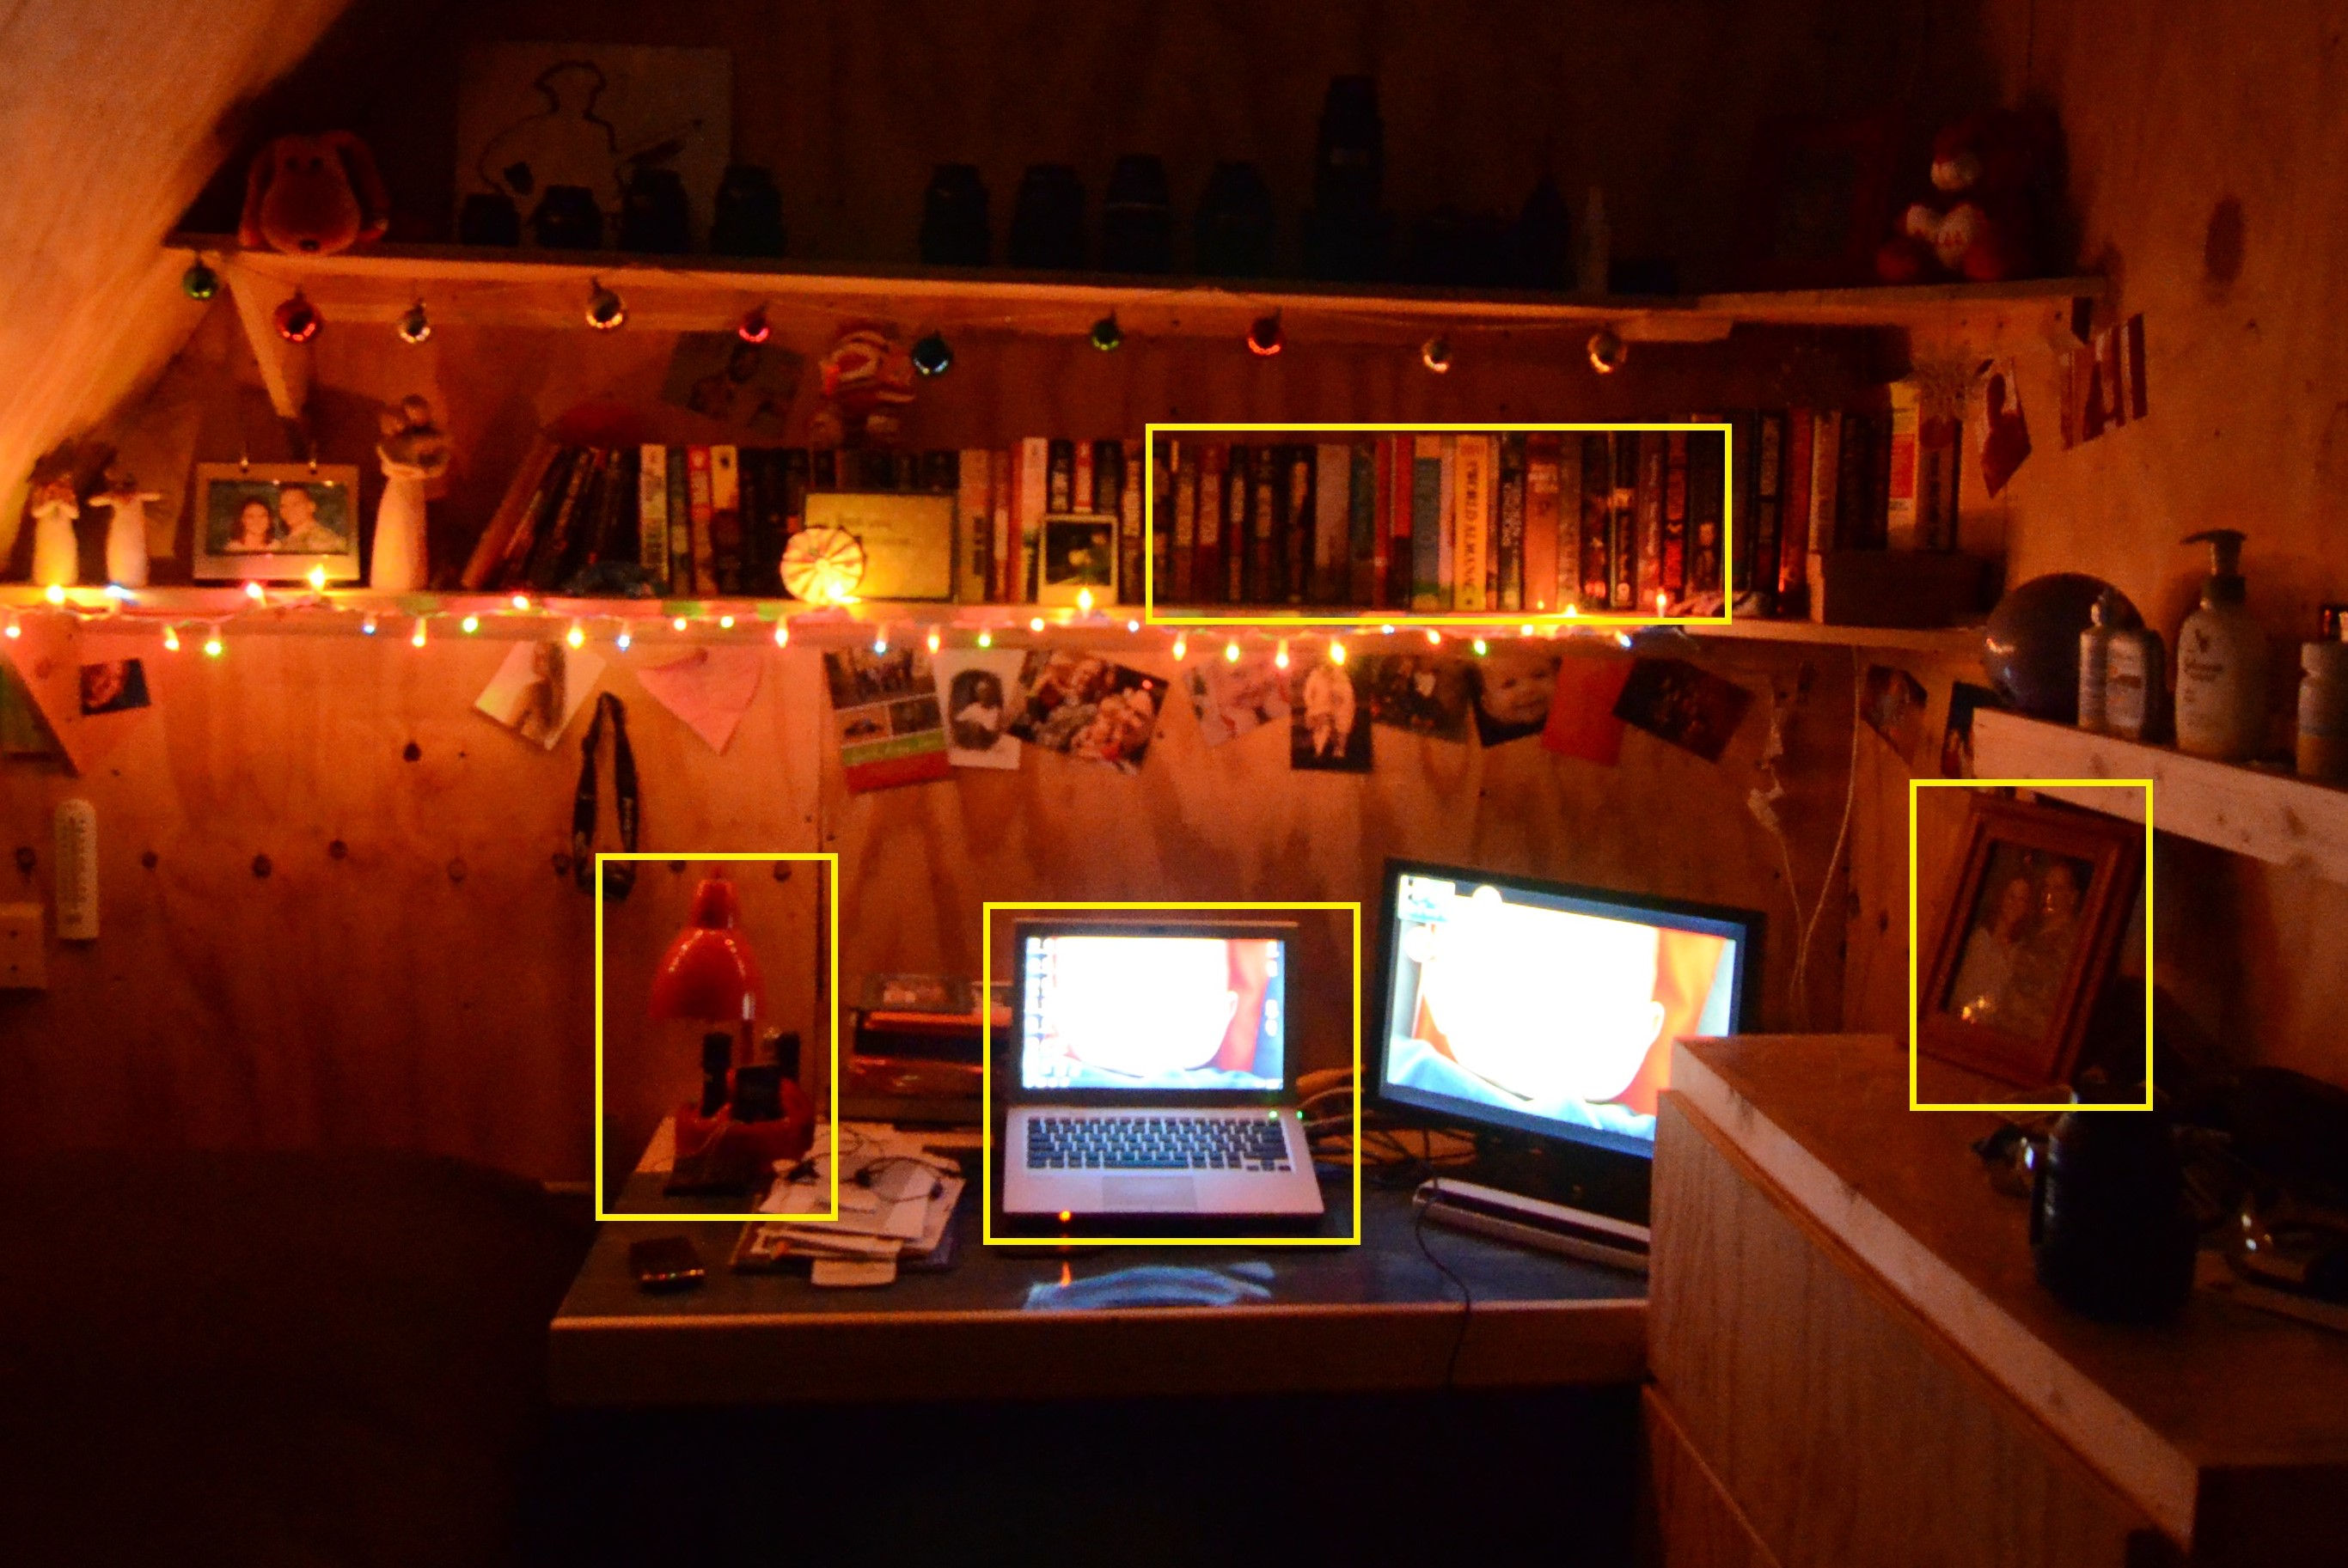
\includegraphics[width=0.95\columnwidth]{dim-room.jpg}
	\end{subfigure}
	\begin{subfigure}{.45\textwidth}
		\centering
		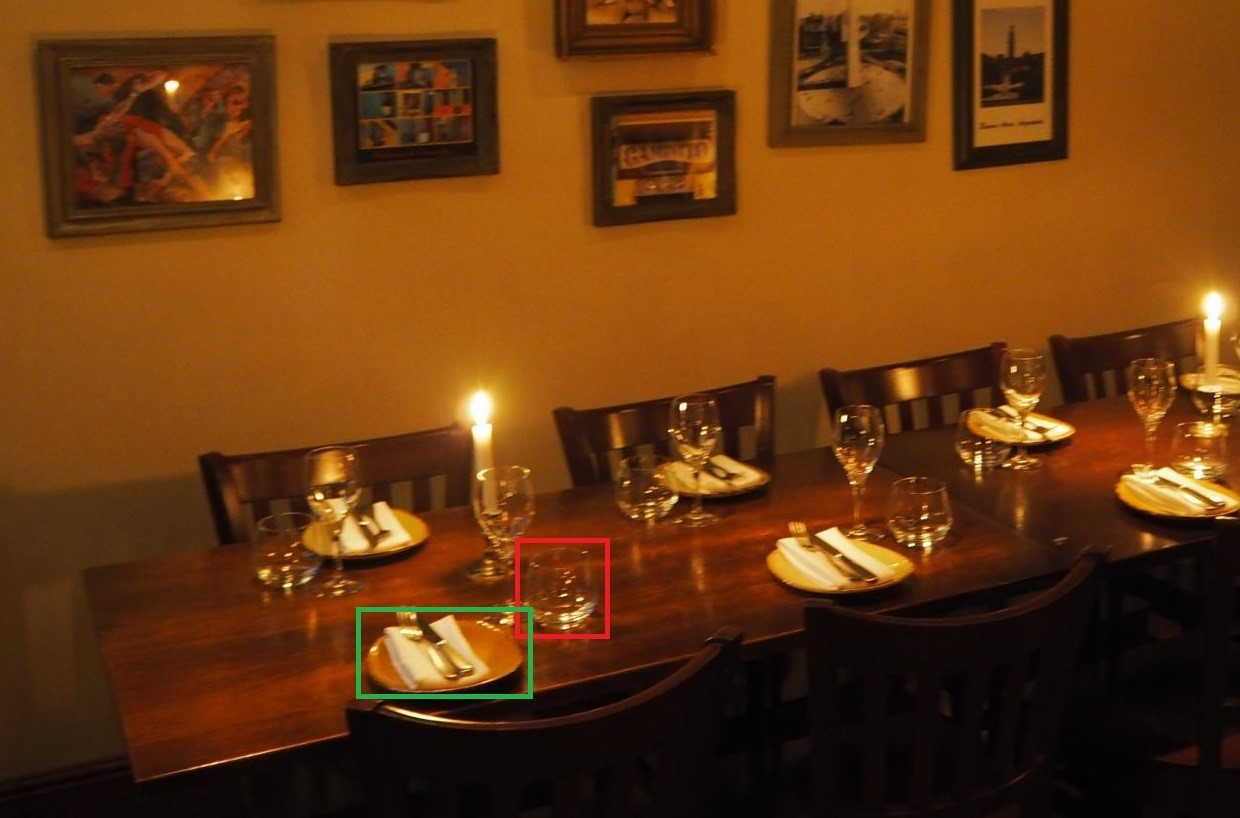
\includegraphics[width=0.95\columnwidth]{dim-table.jpg}
	\end{subfigure}
	\caption{\lnear~relation facts assist the detection of vague objects: in a dimly lit room with settings shown in the \textit{left sub-figure}, if a bright laptop is present on a table, one may guess that a lamp, a photo frame or books maybe nearby. Similarly in the \textit{right sub-figure}, if a set of knife, fork and plate is on the table, one may believe there could be a glass beside based on the commonsense, 
		even though these objects are hardly visible due to low light.}
	\label{fig:dim}
\end{figure}
However, such commonsense knowledge is largely manually curated, therefore it does not scale well and the recall is a serious problem.
For example, ConceptNet contains only 49 \lnear~
relation triples. 
Many commonly co-located objects such as (house, garden) and 
(fork, knife) are not included in this knowledge base. 
Another problem of manually curated data source is that, because manual
annotation is expensive, a pair is typically annotated by just one 
or a few persons. 
As a result, no meaningful statistical confidence scores can be
associated with each triple, which makes ranking-based 
computation using such knowledge base difficult. 
For example, although ConceptNet gives a confidence
score (from 0 to infinity) to each triple, most of the triples are assigned the default
score of 1.
%, simply because the human contributor did not or could not 
%provide a score. 
%If such commonsense knowledge is harnessed automatically
%from open-domain text corpora, both of the above problems can be 
%effectively addressed. 
%Open information extraction not only provides the much needed scale,
%but also valuable statistics that can turn into confidence scores.

In this paper, our goal is to extract \lnear\ relation between
physical objects, which is defined as two objects typically found near each
other.\footnote{Because some physical objects can be a location itself, this
relation may include some instances of the \textsc{atLocation} relation,
e.g., {\em room} and {\em door}.}
We focus on \lnear\ relation for these reasons:
\begin{itemize}
\item Prior knowledge of \lnear\ relations is helpful for object detection in complex image scenes; 
For example, if a bright laptop is present on a table, one may guess that a lamp, a photo frame or books maybe nearby; in a dimly lit restaurant, if some plates are present on a table,
one may guess that wine glasses or other kitchenware maybe nearby, 
even though these objects are hardly visible (see \figref{fig:dim});
\item \lnear~relation can benefit general reasoning in reading comprehension, question answering and many other AI tasks;
\item \lnear~relation extraction itself is a challenging task, as interpreting spatial relations from text is not trivial and many relation mentions are implicit due to figurative language.
\item Existing knowledge bases such as ConceptNet has very limited facts for this relation. Only 49 \lnear~relation assertions are found in current dump of English ConceptNet knowledge base, thus the urgent need for extracting this specific relation.
\end{itemize}



Since \lnear\ relationship is more prevalent in literary work such as stories 
and dramas which come with descriptive scenes rather
than in science \& technology related articles,
we propose to extract it from literature.
However, sentences in literature are often complex and nuanced, 
which makes extraction particularly challenging. 
%Consider the objects
%	``bed'' and ``star'' in the following
%	sentence: ``{\em Until at last all the promenaders had gone home to bed, 
%	and I was alone with the star.}'' Bed is not near the star because it's at another location;
Also, obtaining a large labeled data set is difficult and expensive.

%\BL{add more related work about KBC here, mainly about Xiang Li (TTIC) and Stating the Obvious; to stress that why we are using raw text}

%Since raw text of novels tend to contain many 
%descriptions of  scene in real life, 
%we argue that it is feasible to obtain unseen 
%{\lnear} relations from raw novel text. 


In this paper we propose a two-stage task in solving \lnear\ relation
extraction problem. 
The first subtask is a binary classification problem which identify whether two mentioned entities in a sentence are {\em co-located} with each other in this sentence. 
The second is given the scores of every sentences, how to produce a ranked list of \lnear\
facts to complete knowledge base. Each \lnear\ fact carries a confidence weight
that indicates the typicality of the fact given the evidence from the
text corpus. Notice that two objects that are {\em co-located} 
in a couple of sentences may not mean they have 
the \lnear\ relation as a commonsense. This confidence weight can serve
as a smoothed version of the confidence score in ConceptNet.

To this end, we create two 
benchmark datasets, one with 5,000 sentences, 
each containing at least two physical objects,
and a label of co-location or not; the other consisting of 500 pairs of
object with binary labels, that is whether a pair is \lnear\ or not.   
We also propose several baseline methods to solve the classification task.
The first kind of approaches leverage syntactic features and word embedding
in the sentence in a SVM model. The second kind of approaches are an LSTM
model that takes advantage of word embeddings of the 
two objects and the most relevant sequential information of the sentences 
indicating the co-location, significantly reducing the size of 
parameters. 
%In both approaches,
%we associate a probabilistic score with each pair of objects extracted
%from a sentence. We then aggregate such scores for each unique pair,
%to produce a commonsense knowledge score for this pair.  
%We construct a dataset consisting of \BL{xxx} instances with labels 
%(\textit{True}/\textit{False}) for training our model. 
%Experiments demonstrate that both of the classification methods 
%outperforms the state-of-art approaches on the \lnear dataset.
%\KZ{Need to back up these in the eval.} 

In summary, this paper makes the following contributions: 
\begin{itemize}
	\item We propose two novel tasks for \lnear~ relation extraction.
	
	\item We make public the first annotated dataset for 
	sentence-level \lnear~ relation classification and another labeled dataset for
	\lnear~ knowledge construction. 
	%	\item We propose a bootstrapping framework that automatically generate X times more training data than the initially labeled.
	
	\item We suggest several baseline methods for \lnear~ relation 
	classification task, 
	which compare favorably with the current state-of-the-art
	method for general-purpose relation classification problem. 
	
	\item We extract in total 2,067 new pairs previously not in
	ConceptNet, with a precision of 0.68.
\end{itemize}

